%(BEGIN_QUESTION)
% Copyright 2006, Tony R. Kuphaldt, released under the Creative Commons Attribution License (v 1.0)
% This means you may do almost anything with this work of mine, so long as you give me proper credit

En \textit{varmeveksler} er en metallisk enhet konstruert for å overføre varme mellom to fluid:

$$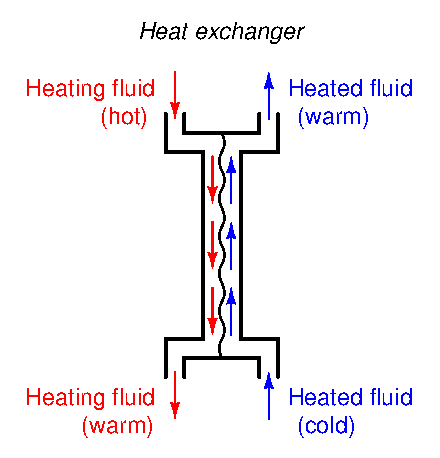
\includegraphics[width=15.5cm]{i00334x01.eps}$$

Et \textit{oppvarmende} fluid går inn på den ene siden av varmeveksleren og avgir noe av sin varmeenergi til det \textit{oppvarmede} fluidet på den andre siden av en tynn metallbarriere. Det oppvarmede fluidet absorberer samtidig varmen som frigjøres fra det oppvarmende fluidet gjennom barrieren, og temperaturen øker før det går ut.

Det finnes mange ulike typer varmevekslere, men alle bygger på de samme grunnprinsippene: termisk konveksjon (varmeoverføring mellom hvert fluid og barrieren) og termisk konduksjon (varmeoverføring gjennom selve barrieren).

Anta at en varmeveksler brukes til å forvarme fyringsolje med damp før forbrenning i en kjel (vanlig praksis i kjelanlegg som bruker tunge flytende petroleumsprodukter, som ``bunker-C''):

$$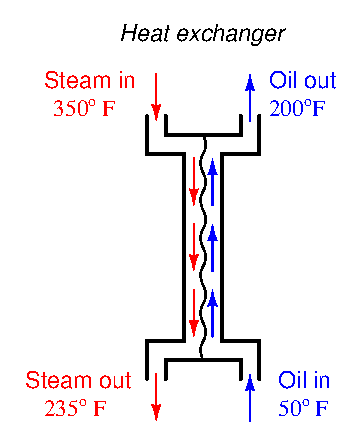
\includegraphics[width=15.5cm]{i00334x02.eps}$$

Hva skjer med utløpstemperaturen til damp og olje dersom \textit{strømningen} av olje reduseres? Gi kvalitative svar (øker, minker eller forblir uendret).


\underbar{file i00334}
%(END_QUESTION)





%(BEGIN_ANSWER)

Hvis oljestrømmen reduseres, vil oljens utløpstemperatur øke fordi hvert oljemolekyl oppholder seg lenger inne i varmeveksleren og dermed rekker å absorbere mer varmeenergi fra dampen.

Dampens utløpstemperatur vil også øke, fordi redusert oljestrøm ikke trekker ut like mye varme fra dampen under passasjen. En måte å se dette på er å tenke at oljen kjøler dampen, snarere enn at dampen varmer oljen. Med mindre olje inn i veksleren for å kjøle dampen, blir utgående damptemperatur høyere enn før.

%(END_ANSWER)





%(BEGIN_NOTES)


%INDEX% Physics, heat and temperature: heat exchangers

%(END_NOTES)
